Applying information theoretical algorithms on a high density EEG dataset is the main focus of this thesis. The EEG dataset is provided by the lab of computational neuroscience of KU Leuven. In order to perform an analysis of a dataset, it is important to understand what kind of data we are dealing with.

This chapter discusses the experiment used to generate the dataset. The experiment and the reasons behind the experiment are introduced. Afterward the actual experiment is discussed. This starts with the an explanation of the EEG experiment itself and the paradigm. Afterwards the source localization is discussed. Finally, the final structure of the data is brievely discussed.

\section{Introduction}

The experiment resolves around the human brain's representation of semantic categories. By using high density EEG recordings, the semantic processing of words within the human brain was captured. Within the literature, there are several different theories and concepts that explain the representation of semantic categories within the human brain. The human brain is a complicated organ with many different cortical areas. Each theory focusses on different cortical areas and explain how they are involved with the representation of semantic categories. These theories have been further developed with the aid of different neuroimaging experiments. 

One of the most prominant theories of semantic word processing is the grounded cognition model. The model is also called the embodied cognition model. This model explains that semantic knowledge is kept within high-level perception and motor representation systems in the brain. 

This means that a word is comprehended based on modality-specific neural systems. In other words, elements such as visual and auditory features are used to define words. As an example, animate objects cluster in the more lateral aspect of the fusiform gyrus, whereas activations associated with inanimate or man-made objects cluster in the more medial aspect of the fusiform gyrus \cite{landrum2015clinvar}. There are other studies that show that damage to the brain's modal system creates category-specific deficits \cite{barsalou2003grounding, caramazza2003organization}. 

These deficits can be explained by using the grounded model, natural objects such as animals, vegetation, etc, are distinguished primarily from their visual semantic properties. On the other hand, man-made objects such as tools and vehicles are distinguished primarily by their function. This is also shown by fMRI and PET imaging studies \cite{devlin2002there}.

The grounded cognition model can be criticized from several aspects. Stimuli that are conceptual in nature are much more difficult to control, as the associated brain activity is almost completely subject-dependent \cite{kemmerer2015visual}. Most importantly, the grounded cognition model only explains features that are related to a physical object. More abstract concepts, such as concepts related to emotions, are not explained by the model. 

Looking at the difference in the processing of abstract and concrete words, there are some theories. The main theories are the dual coding theorem and the context availability theorem \cite{kounios1994concreteness, wang2010neural}. The dual coding theorem states that there are two separate systems within the brain, a nonverbal "imagery" system and a verbal "linguistic" system. The nonverbal system implement is very alike to the grounded cognition model. The verbal system is involved with the abstract nature of language.

The context availability theorem is quite different from the dual coding theorem. Rather than having two distinct systems, the context availability theorem states that the processing of concrete and abstract words never happen in isolation and that context is important. Context determines how words are processed. Concrete words are contextually related to their physical referents. Abstract words are more variable and are contextually related to previous experience. 

Neither theory has been proven or disproven by scientific literature. Most research into these theories have been done using functional neuroimaging techniques such as fMRI and PET, which is limited in terms of temporal resolution \cite{bookheimer2002functional}. EEG, by virtue of its excellent temporal resolution, has become popular to probe the brain's detailed processing of objects and words. Several studies using EEG/ERP recordings have successfully distinguished different word categories. This has been done on different stages of semantic processing \cite{hauk2006time}. One disadvantage to using EEG is the low spatial resolution, which makes it fall short in detecting cortical network activiation differences. 

In the experiment described in this chapter, high density EEG recordings were used to capture the fast dynamics involved in semantic processing. The neural activity has been localized on the cortex with an accuracy in the range of millimetres and milliseconds. This provides an interesting and unique opportunity to analyse the activity during the semantic processing of abstract and concrete words.

\section{Materials and methods}

The experiment was done in a sound-attenuated, darkened room with a constant temperature of 20 degrees, sitting in front of an LCD screen at a distance of about 70cm.

EEG data is recorded using 128 active Ag/AgCl electrodes (SynampsRT, Compumedics, France), according to the international 10-20 system. Two of these electrodes serve as ground (AFz) and reference (FCz). The EEG signal is recorded at a 2 KHz sampling rate and downsampled to 500 Hz. All electrodes are mounted in an electrode cap that is placed on the subject's head (Easycap, Germany). 

\section{Experimental Paradigm}

Choosing the correct paradigm is important. The paradigm has to make sure that the subjects are involved in lexical access and semantic processing. Therefore, a categorization paradigm was selected. This paradigm consists out of 600 Dutch words, all of which are nouns, taken from the database of concreteness ratings for 30,000 Dutch words \cite{brysbaert2014concreteness}.

These words are split up into two groups, abstract and concrete words. Abstracts words have a concreteness rating of maximum 2.5, and concrete words have a concreteness rating of minimum 3.5. The concreteness rating of abstract and concrete words are statistically different, as tested by a t-test.

Both groups are controlled for word length and word frequency, having no significant difference. Word length and word frequency are computed from the Dutch CLEARPOND software. The words are also pseudo randomly organized in order to make sure that no two consecutive words have a high forward association, and forward associations is controlled for all consecutive words. Forward associations was taken from the Dutch free association network created by De Deyne et al \cite{de2008word}. 

Figure~\ref{experiment} shows the general flow for each trial. In each trial, a single word in white text is presented on a fully black screen. The word is shown for 300ms. This is followed by a question mark that is shown for a duration of 1 second. Each trials starts by showing a fixation cross to cue subjects to focus on the middle part of the screen. 

Subjects are asked to press the mouse button as soon as they the question mark and the word they are shown is a colour. The colour category is used as a non-target, or filler, and are not included in the results. After the button press, the subjects are given visual feedback on the button press. They are shown "kleur!" (colour) if they pressed correctly, and "fout!" (wrong) otherwise.

\begin{figure}[!htb]
\caption{General Flow for each Trial.}
\label{experiment}
    \centering
    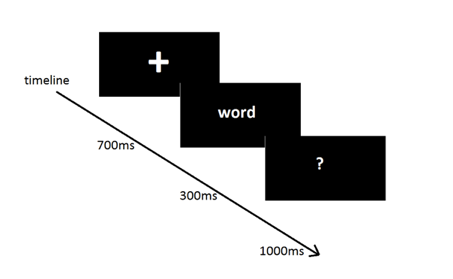
\includegraphics[width=\textwidth]{fig/experiment}
\end{figure}

\section{Source localization}

In order to source reconstruct the EEG data, the Brainstorm toolbox is used \cite{tadel2011brainstorm}. The Brainstorm toolbox is freely available under the GNU general public license. The default anatomy is based on the ICBM-152 template.

OpenMEEG BEM model is used for the forward model \cite{gramfort2014mne}. In this model, the cortex is divided into 15,000 dipoles. By merging the matrices computed from the baseline of all selected trials, the noise covariance and data covariance matrices are obtained. 

Section~\ref{source-alg} discussed different algorithm that can be used for the inverse modelling method. In this case, sLORETA is used \cite{pascual2002standardized}. sLORETA yields zero localization error. Source orientation is constrained to be orthogonal to the cortical surface. The signal-to-noise ratio (SNR) is kept at the default suggested value, which is 3. Sulci are not taken during the analysis. Brainstorm's documentation states that accurate source localization in these regions is implausible.

Using different source localization algorithms, the correctness of the procedure is verified \cite{mahjoory2017consistency}. The results are analysed by taking the average over all trials regardless of semantic features, using the four methods available in the brainstorm toolbox: wMNE, dSPM, sLORETA, and unconstrained sLORETA.

\section{Region of Interest selection}

In order to be able to focus on a very specific set of data, the delivered data only contained several regions of interest. The procedure for selecting the regions of interest starts from the source reconstructed data, obtained by using sLORETA. The current density maps were normalized with respect to a reference level in order to provide a statistical map. This statistical map is essentially the signal to noise ratio of the current estimate as a function of location. The normalized source maps are used to evaluate the significance of the data. 

The sLORETA statistical maps are averaged over all trials and activity below 75\% of the maximum activity is eliminated. This is done for both paradigms (abstract and concrete). The two obtained maps are overlapped and from this the most active regions with an estimated square size of larger than 3cm$^2$ are selected. This resulted in four regions on the inferior temporal gyrus, temporal pole, inferior frontal, and anterior orbital gyrus. Figure~\ref{experiment-2} visualizes the selected regions.

\begin{figure}[!htb]
\caption{Visualization of the Selected Brain Regions.}
\label{experiment-2}
    \centering
    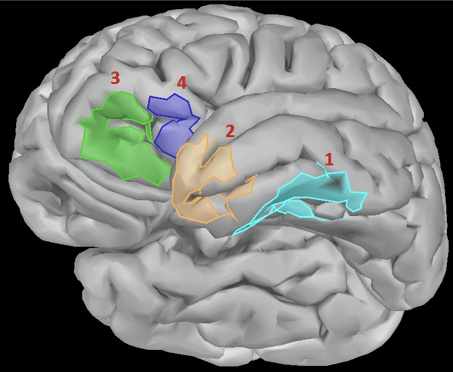
\includegraphics[width=\textwidth]{fig/experiment-2}
\end{figure}
